% ===== INICIO DEL PREÁMBULO =====
%
\documentclass[msc,oneside,a4paper]{udelar} % Poner msc para Maestría, dsc para Doctorado.
%
\usepackage[
acronyms, %utiliza el glosario de acronimos.
nohypertypes={acronym,notacion,simbolos,glosario}, %quita los links en el texto al glosario.
%nonumberlist,                                       %quita los links en los glosarios al texto.
nogroupskip, %quita los espacios entre diferentes grupos dentro de un glosario.
nopostdot, %quita el punto final en los acrónimos
]{glossaries}

\hypersetup{colorlinks=false,pdfborder={0 0 0}} % Hipervínculos: escribir "false" para imprimir o "true" para ver en digital.

% Ver los documentos de estilos bibliográficos para editar estas siguientes 2 líneas. Se deben de copiar a partir de los PDF de estilos bibliográficos y no es necesario que el estudiante las edite.
\usepackage{natbib} % Para algunos estilos bibliográficos
\bibliographystyle{estilos_bibliograficos/natbib/apalike}

\loadglossary 

% A su vez, la clase udelar.cls ya tiene los siguientes paquetes cargados automáticamente, que podrían ser de interés saber para el usuario:
% 
% {color},{hyphenat},{appendix},{lastpage},{babel},{inputenc},{amsmath,amssymb},{ifthen},{graphicx},{caption}
% {setspace},{tabularx},{eqparbox},{ltxcmds},{titletoc},{xcolor},{lineno},{xwatermark}

% Si se quieren agregar más paquetes, se recomienda colocarlos a partir de esta linea y antes de \begin{document}.
% ===========  INICIO PAQUETES ===============

\usepackage{booktabs}
\usepackage{placeins}

% ===========   FIN PAQUETES   ===============

\newcommand{\modelspace}{\hspace{1.5em}}

% =====  FIN DEL PREÁMBULO  =====

% ===== INICIO DEL DOCUMENTO =====

\begin{document}
  %
  \title{Diseño de redes de ciclovías enfocado a la atracción de demanda}
  % \subtitle{Subtítulo de la tesis}
  \institutelogo{0} % Carga cantidad de logos seleccionados, con máximo de 3 logos.
  \author{Joaquín}{Correa}
  \escritura{Investigación de Operaciones}
  %
  \director{Prof.}{Antonio}{Mauttone}{Dr.}
  \director{Prof.}{Franco}{Robledo}{Dr.}
  \directoracademico{Prof.}{Franco}{Robledo}{Dr.}
  %
  \examiner{Prof.}{Nombre del 1er Examinador}{Apellido}{D.Sc.}
  \examiner{Prof.}{Nombre del 2do Examinador}{Apellido}{Ph.D.}
  \examiner{Prof.}{Nombre del 3er Examinador}{Apellido}{D.Sc.}
  %
  \graduatename{}
  \institute{Facultad de Ingeniería}{FIng}
  \graduatelocation{Montevideo}{Uruguay}

  \date{20}{07}{2022}

  % Palabras claves en español
  \keyword{diseño de redes}
  \keyword{ciclovías}
  \keyword{transferencia de demanda}
  \keyword{optimizacón}

  \maketitle
  \frontmatter  % Comando que genera la portadilla, el catalogo y el tribunal de evaluación. NO COMENTAR

  \include{misc/dedicacion}
  % \chapter*{Agradecimientos}

Quisiera agradecer a...

  % \include{misc/epigrafe}
  \begin{abstract}
    La modalidad de transporte urbano utilizando bicicleta puede traer beneficios tanto en la salud y bienestar de las personas como para la ciudades disminuyendo la congestión del tráfico, mejorando la calidad del aire y reduciendo la contaminación sonora. Quienes están a cargo de las decisiones sobre la gestión del espacio público en ciudades (municipalidades, intendencias) pueden realiza acciones para que más personas realicen sus viajes habituales en bicicleta. Un tipo de acción es la construcción de infraestructura para circular en bicicletas, también conocidas como ciclovías. Las infraestructuras se pueden construir sobre la red de calles de una ciudad formando una red de ciclovías, estas pueden ser de varios tipos o tecnologías y afectan la experiencia de usuario de manera que a mejor experiencia mayor costo de construcción tienen. Asumiendo que se conoce la demanda origen-destino potencial de viajes en bicicleta que actualmente utiliza otro medio de transporte, que se cuenta con un presupuesto acotado para construir ciclovías y que más personas van a utilizar bicicleta si cuentan con más y mejor infraestructura específica de ciclovías, en esta tesis estudiamos el problema de maximizar la atracción de demanda hacia la bicicleta desde otros medios de transporte mediante la decisión de dónde y qué tipo de ciclovías construir. Lo modelamos como un problema de optimización en redes, mediante una formulación de programación matemática no lineal que luego reformulamos para obtener una formulación lineal entera mixta (MILP). El problema resultante se resuelve con técnicas de resolución MILP del estado del arte que probamos numéricamente con una instancia tomada de la literatura y una construida en base a datos de la ciudad de Montevideo.
\end{abstract}



%  \listoffigures	         % Lista de figuras
%  \listoftables	         % Lista de tablas
%  \listadesimbolos 		     % Lista de símbolos
  %\listadenotaciones 	     % Lista de notaciones
  % \listadesiglas 		     % Lista de siglas
  %
  \tableofcontents
  \mainmatter % Comando que genera las listas y capítulos. NO COMENTAR

  % Se incluyen los capítulos. Se pueden comentar los capítlos en los cuales no se está trabajando, para que el documento de trabajo sea más pequeño y compile más rápido.
  \chapter{Introducción}

  Utilizar la bicicleta como medio de transporte brinda un amplio espectro de beneficios. Es una alternativa particularmente favorable para viajes cortos en comparación al uso de automóvil o transporte colectivo \parencite{Hull2014}. La sustitución del transporte motorizado por bicicleta es favorable para el descongestionamiento de calles y la consiguiente disminución en la contaminación sonora y del aire, problemas que son comunes en ciudades medianas y grandes. En Uruguay, una proporción significativa de la población padece enfermedades no transmisibles asociadas a la inactividad física como enfermedades cardiovasculares y obesidad; está demostrado que la práctica de ejercicio frecuente de moderada intensidad como el transporte en bicicleta, junto a otros cambios en el estilo de vida, previene el desarrollo de los factores de riesgo más prevalentes \parencite{heartrisksuy, mspphisicalactivityguid, mspsurveyriskfactors}. Sin embargo, a pesar de las ventajas citadas anteriormente, no siempre es posible utilizar este medio de transporte debido a factores como la distancia del viaje, condiciones climáticas adversas y falta de infraestructura adecuada, entre otros.

  Si bien la bicicleta puede utilizar la red de calles o incluso sendas peatonales como medio de circulación, no siempre estas son elegibles por los ciclistas para su uso. Factores como la cantidad y velocidad del tránsito automotor y ancho de la banquina afectan considerablemente esta decisión. La necesidad de infraestructura específica para la bicicleta es ampliamente reconocida y un correcto diseño es clave para la aplicación eficiente de políticas públicas que busquen mejorar e incentivar la bicicleta como medio de transporte alternativo \parencite{Hunt2007}.

  Según la última encuesta de movilidad realizada para el área metropolitana de la ciudad de Montevideo \parencite{Mauttone2017a}, la utilización de la bicicleta abarca el 2,6\% del total de los viajes diarios. Se desprende de dicho estudio que que la bicicleta es el medio de transporte privado de distribución más equitativa, por su presencia en similares valores entre hogares de diferentes estratos socioeconómicos. En Latinoamérica, la utilización de la bicicleta no dista mucho del caso de Montevideo (ver Tabla \ref{table:bicycleusagelatinamerica}) y en general está lejos de los niveles que se pueden ver en otras partes del mundo. Podemos encontrar valores altos en el porcentaje de utilización de la bicicleta en algunas ciudades de Europa que cuentan con buenos niveles de servicio en ciclovías, por ejemplo Cambridge, Reino Unido, con 20\%; Amsterdam y Utrecht, Holanda con 37\% y 44\% respectivamente \parencite{Hull2014}; y Copenhague, Dinamarca con el 35\% \parencite{Vedel2017}. Por otro lado, algunas ciudades de China cuyo medio de transporte predominante ha sido la bicicleta, llegando a niveles superiores al 50\% a principios de este siglo, están viendo decrecer su utilización a razón de 1\% anual en promedio \parencite{Li2017}.

  \begin{table}[h!]
    \centering
    \begin{tabular}{lcr}
      \toprule
      País & Ciudad & \shortstack{Viajes en bicicleta (\%)} \\
      \midrule
        Argentina & Buenos Aires & 3,0 \\
        Argentina & Rosario & 5,3 \\
        Brasil & Río de Janeiro & 3,2 \\
        Brasil & San Pablo & 1,0 \\
        Chile & Santiago de Chile & 3,0 \\
        Chile & Validivia & 2,0 \\
        Colombia & Bogotá & 5,0 \\
        México & Mexico D.F. & 2,0 \\
        Peru & Lima & 0,3 \\
        Uruguay & Montevideo & 2,6 \\
      \bottomrule
    \end{tabular}
      \caption{Porcentaje de viajes en bicicleta sobre el total de viajes realizados en un día típico para algunas ciudades de Latinoamérica \textcite{Idb2020}.}
      \label{table:bicycleusagelatinamerica}
  \end{table}

  La toma de decisiones que lleva a un buen diseño de una red de ciclovías es problema complejo influido por múltiples factores como las características topológicas de la ciudad, la demanda de viajes, el presupuesto disponible y el comportamiento de los usuarios. Desde la optimización podemos encontrar herramientas que ayudan y dan soporte a estas decisiones.

  \section{Conceptos y estado del arte}

  % Orden de las cosas:
  % - Definiciones
  % - Casos de estudio de transporte en bicicleta
  % - Casos de estudio de transferencia de demanda
  % - Casos de estudio del comportamiento de los usuarios

  % ---Definiciones

  La planificación de ciclovías es un problema conocido en el área de Investigación Operativa y ha sido tratado de varias formas. Al igual que otros problemas del área de transporte urbano, el marco de trabajo es una red que representa un área geográfica, por ejemplo la red de calles de una ciudad donde los nodos representan la intersección de calles y los arcos cada segmento de una calle que une un par de intersecciones; una matriz origen-destino que especifica la demanda de viajes (o usuarios que viajan) entre pares de nodos de la red y se consideran diferentes costos, como el costo percibido por cada unidad de demanda al atravesar un arco de la red (típicamente, distancia o tiempo) y el costo de las instalaciones que se pueden construir sobre arcos y nodos de la red (típicamente, costo monetario). Las instalaciones pueden ser infraestructura de ciclovía, estacionamientos o {\it dock stations} para los sistemas de bicicletas compartidas. A diferencia de otros medios de transporte, en este tipo de problemas se puede considerar que la red subyacente es transitable por los ciclistas sin necesidad de instalaciones específicas. En otras palabras, en una ciudad sin infraestructura específica de ciclovías, se puede asumir que es posible circular en bicicleta utilizando la red de calles, compartiendo espacio con vehículos motorizados. A continuación describimos los trabajos más significativos en metodologías de optimización aplicadas al diseño de ciclovías, modelado de transferencia de demanda, modelos de comportamiento de usuarios y técnicas generales de optimización de redes de transporte.

  % ---Transporte en bicicleta
  % Ordenado por año
  % - Taylor1999, Buehler2016: La relevancia de modelar el problema de planificación de ciclovías como un problema de redes de transporte ha sido
  % resaltado por ....
  % - Lin2013: Uno de los primeros trabajos que afronta el problema de diseño de ciclovías. Es un modelo multiobjetivo cuyos cuatro objetivos son: que minimiza el riesgo de los ciclistas, maximiza su confort, maximiza la cobertura del servicio y minimiza el impacto de las ciclovías en el tráfico. La formulación resultante es compleja, considera tres tipos de infraestructuras de ciclovías y fue aplicada a una región de la ciudad de Taipei modelada como una red de 75 nodos y 115 arcos, resuelta utilizando un solver comercial. La inaplicabilidad de esta formulación a regiones más grandes esta dada,dicen, por la dificultad en el manejo de los datos y no necesariamente por la complejidad.
  % - Duthie2014: Buscan, minimizando el costo de construcción de ciclovías en arcos y nodos, conectar todos los pares origen-destino con caminos cubiertos por ciclovías restringiendo el desvío en el largo del camino respecto al camino más corto. Utilizaron un único tipo de infraestructura y resolvieron de forma óptima utilizando un solver MILP comercial una red que modela la ciudad de Austin, Texas con 75 nodos y 185 arcos utilizando 5,625 pares origen-destino.
  % - Mauttone2017, baya2021:
  % - Liu2019: Planten un modelo binivel que maximiza la utilidad de los ciclistas, sujeto a presupuesto, que se trasladan según una matriz origen-destino. El segundo nivel representa el comportamiento de los usuarios mediante un modelo logístico en función un escalar que captura los factores que afectan a los ciclistas en sus decisiones: largo de la ruta, frecuencia de curvas, pendiente y presencia de ciclovía. Para resolver el modelo primero fue reformulado con lo que pudieron resolver instancias medianas con solvers MILP comerciales. Para resolver instancias grandes desarrollaron una heurística que achicaba la región factible del problema y asi resolverlo con un solver ya mencionado.
  % - lim2021: mencionar trabajo pero por arriba diciendo que no esta revisado.

  En \textcite{Lin2013} podemos encontrar uno de los primeros trabajos publicados que afrontan el problema de diseño de ciclovías como un problema de diseño de redes. Plantean un modelo multiobjetivo que minimiza el riesgo de los ciclistas, maximiza su confort, maximiza la cobertura de las ciclovías y minimiza el impacto en el tráfico. Consideran tres tipos de tecnologías de ciclovía. La formulación resultante es un problema lineal entero mixto (MILP) y fue aplicada a una región de la ciudad de Taipei, China, modelada como una red de 75 nodos y 115 arcos, resuelta utilizando un solver MILP comercial. En \textcite{Duthie2014} se propone un modelo que busca minimizar el costo de construcción de ciclovías en arcos y nodos dado que todos los pares origen-destino están conectados por caminos en los que hay ciclovía y restringiendo el desvío en el largo de los caminos sobre la ciclovía respecto a un factor multiplicado por el largo del camino más corto sobre la red de calles. Utilizaron un único tipo de tecnología de ciclovía y resolvieron de forma óptima utilizando un solver MILP comercial una red sobre la ciudad de Austin, Texas con 75 nodos y 185 arcos, utilizando 5625 pares origen-destino. Más tarde, \textcite{Mauttone2017} introduce un modelo MILP que, mediante la construcción de infraestructuras de ciclovías que reducen el costo de usuario de atravesar los arcos en los que se construyen, minimiza la suma de los costos de usuario de trasladarse por el camino más corto. En este trabajo se utilizó un único tipo de tecnología de ciclovía y se logran resolver optimamente instancias pequeñas utilizando un solver comercial por lo que propusieron una metaheurística GRASP para resolver instancias grandes. Incluyeron en el GRASP un parámetro para penalizar la discontinuidades de las ciclovías, entendiéndose como discontinuidad la cantidad de veces que un usuario sale de la red de ciclovías (hacia la red de calles) durante su recorrido. Luego, en \textcite{baya2021} se estudia un problema similar pero considerando múltiples tipos de tecnologías de ciclovías y las discontinuidades dentro de un modelo de programación matemática. Logran resolver óptimamente utilizando un solver MILP comercial una red que modela la ciudad de Montevideo con 136 nodos y 636 arcos. En \textcite{Liu2019} se plantea un modelo binivel donde el primer nivel maximiza la utilidad de los ciclistas que se trasladan según una matriz origen-destino, sujeto a presupuesto. El segundo nivel representa el comportamiento de los usuarios mediante un modelo logístico en función del valor de utilidad percibida por los usuarios, éste es un valor escalar que captura los factores que afectan a los ciclistas en sus decisiones: largo de la ruta, frecuencia de curvas, pendiente y presencia de ciclovía. Para resolver el modelo primero fue reformulado en un MILP con lo que pudieron resolver instancias medianas con solvers comerciales. Para resolver instancias grandes desarrollaron una metaheurística que reduce la región factible del problema para luego ser resuelto con el mismo MILP que habían desarrollado. Mientras tanto en \textcite{lim2021}\footnote{Este trabajo no se encuentra publicado pero si disponible en \url{https://arxiv.org/abs/2107.04451}} se propone un modelo en el que se planifica la red de ciclovías considerando que la demanda puede ser satisfecha si existe un camino de ciclovías que conecta el origen y el destino; y el desvío sobre el camino más corto sobre la red de calles no supera un umbral. El modelo minimiza la penalización sobre el valor de desvío que se modela en la función objetivo como una función lineal de a partes. Logran resolver una instancia que modela la calles de una sección de la ciudad de Atlanta, Estados Unidos, con 5815 nodos y 11329 arcos, utilizando el algorítmo de descomposición de Benders.

  % ---Transferencia de demanda: Los que menciono son todos iguales
  %
  % - garcia2005: Donde construir lineas de metro y estaciones para que la mayor cantidad de demanda use el tren. Mismo problema que el mio pero para trenes. Transferencia modelada como all-or-nothing.
  % - laporte2007:
  % - marin2007:
  % - cadarso2015: (igual a los 3 anteriores)

  La transferencia de demanda entre modos de transporte, entendida como el proceso en el cual los usuarios deciden cambiar el modo de transporte para trasladarse entre dos puntos, ha sido un tema abordado principalmente de dos maneras en la literatura: con modelos determinísticos mediante los cuales la demanda se transfiere entre modos dependiendo de un valor en el costo o utilidad de los usuarios; y modelos probabilísticos en los que dependiendo de la utilidad de utilizar cada modo de transporte obtenemos su probabilidad de utilización y en base a esto un valor de demanda que utiliza cada medio. Sobre los primeros. múltiples publicaciones han estudiado problemas de optimización en la demanda que se transfiere a cierto medio de transporte en función del costo de usuario. Este es el caso en \textcite{garcia2005} y \textcite{laporte2007} en los que tratan distintas variantes del {\it Rapid Transit Network Design Problem} o diseño de redes aplicado al transporte de metro y trenes en los cuales se planifican las líneas y estaciones a construir para satisfacer la mayor demanda posible. El objetivo en estos trabajos es maximizar la cobertura de viajes por parte de la red de trenes. En este caso el término cobertura de viajes refiere a la demanda que puede ser satisfecha por la red que está siendo diseñada en lugar de que ésta utilice transporte privado, por lo que el concepto es equivalente a lo que entendemos por transferencia de demanda. El modelado de la cobertura de demanda se realizó como {\it all-or-nothing}, lo que significa que si el costo de usuario de ir de un origen a un destino utilizando la red es menor a un valor umbral dado como parámetro para dicho par origen-destino, entonces se considera que la demanda de ese par origen-destino está cubierta. En estos problemas los usuarios solo se pueden trasladar por arcos y nodos donde hay líneas y estaciones de trenes activas y se maneja un parámetro de congestión que modela la capacidad de los trenes. A su vez hay límites de presupuesto para el costo total de las instalaciones y límites en el largo de las líneas. Los problemas fueron formulados como MILP y resueltos utilizando solvers comerciales. Luego, en \textcite{marin2007} y \textcite{cadarso2015} se formulan problemas similares pero multiobjetivos. En el primero se agrega el objetivo de minimizar el costo total de los trayectos y en el segundo se agrega a lo anterior la minimización de los costos de las instalaciones.

  Por el otro lado, sobre los modelos probabilísticos del modelado de transferencia de demanda podemos encontrar en el libro {\it Modeling Transport} \textcite{ortuz2011} la definición de modelos de elección discreta (DMC, en inglés). En estos modelos se define el concepto de utilidad un individuo de utilizar un medio de transporte y se define en función de variables o indicadores que tomen en cuenta cualquier tipo de información trascendente al problema sobre el individuo y el trayecto, por ejemplo: nivel socioeconómicos, disponibilidad de vehículos, tiempo de viaje en bici, etc; y se le suma un componente aleatorio de media 0 que modela lo que escapa al modelado. Luego, para determinar la probabilidad de utilización de un individuo sobre los diferentes modos de transporte se utilizan transformaciones matemáticas que lo permitan como los modelos logístico y probit. Por ejemplo, la probabilidad de que un individuo utilice la bicicleta para su traslado en lugar de hacerlo por transporte privado o bus, siendo las utilidades $U_{bici}, U_{auto}$ y $U_{bus}$, utilizando el modelo logístico, es: $P_{bici} = {e^{U_{bici}} \over {e^{U_{auto}} + e^{U_{bus}}}}$. En \textcite{Pacheco2021} proponen un método por el cual se puede integrar DMC a un MILP siempre y cuando las funciones de utilidad sean lineales asumiendo que sus variables también son variables del MILP. El método propuesto permite obtener un valor de la demanda esperada que utiliza cada medio de transporte mediante la inclusión de valores sorteados del componente aleatorio de las funciones de utilidad al juego de parámetros del modelo MILP. Esto funciona siempre y cuando el objetivo del MILP esté en función de las variables de las funciones de utilidad o de la demanda esperada.

  Continuando con los modelos probabilísticos tenemos el enfoque utilizado por \textcite{Liu2019} que aborda el problema de diseño de ciclovías. Definen un MILP con múltiples pares origen-destino y múltiples caminos precomputados entre cada par origen-destino. Asumen que toda la demanda se traslada en bicicleta y el objetivo es maximizar la utilidad total de la demanda sobre todos los caminos. El cálculo de demanda que usa cada camino se realiza en base a la probabilidad de utilizarlo que depende de la utilidad percibida. La utilidad de un par origen-destino sobre cada camino está compuesta por una utilidad fija del camino (parámetro del modelo) y una utilidad variable que depende de la presencia de ciclovías en los arcos del camino. Luego se calcula la demanda esperada sobre cada camino mediante el producto de la demanda total para el par origen-destino por la probabilidad de utilización del camino en lugar de los otros caminos para el par origen-destino. La probabilidad de utilizar cada camino es calculada utilizando un modelo logístico que involucra el valor de utilidad percibida antes mencionado junto a un factor, conocido como {\it path-size}, que penaliza rutas que comparten arcos con otras rutas. Este tipo de modelos se conocen como modelos {\it path-size logit} (PST).

  % ---Comportamiento de los usuarios

  El comportamiento de los ciclistas respecto a las decisiones que toman para trazar un camino entre dos puntos se ha analizado en varios trabajos mediante encuestas. A diferencia del transporte vehicular que se sensible al flujo, es decir, el tiempo de viaje es una función creciente del flujo de vehículos, el transporte en bicicleta considera otros factores en la elección de rutas como la seguridad y la presencia de ciclovías. El efecto de la congestión no es un factor significativo en la elección de rutas \parencite{broach2012}. En el estudio \textcite{winters2010} se analiza una encuesta a ciclistas y potenciales ciclistas en Vancouver, Canadá comparando las rutas utilizadas por estos y la ruta más corta en distancia. Encontraron que el 75\% de los viajes en bici estaban dentro del 10\% del camino más corto (factor de desvío $< 1.1$) y el 90\% dentro del 25\% del camino más corto. Si bien estos valores fueron similares para el transporte vehicular, el desvío fue un poco más acentuado para los ciclistas. También se observó que hubieron factores de desvío menores a 1 para algunos ciclistas que utilizaron sendas o vías no transitables. Comparado con los caminos elegidos, los ciclistas pasaron significativamente menos tiempo en vías arteriales y significativamente más tiempo en vías vecinales o con presencia de infraestructura de ciclovía.

  En \textcite{shwe2014} se realiza una encuesta en Europa analizando el potencial de viajes en bicicleta comparándolo con la situación al momento del trabajo. Fijan un umbral de 5 km y consideran que todos los viajes cuyo trayecto es menor a dicha distancia son realizables en bicicleta. Como resultado estiman que, en promedio, la mitad de los viajes podrían ser realizados en bicicleta. Sin embargo, el porcentaje de encuestados que cambiaría su modo de transporte a la bicicleta asumiendo un escenario en donde el mejor tipo de tecnología de ciclovía está disponible de manera continua en todas direcciones y se cuenta con estacionamientos para bicicletas suficientes, es mucho menor al valor potencial anteriormente mencionado. Esto implica, aseguran, que las políticas de construcción de ciclovías deben ser acompañadas de medidas complementarias de promoción y educación sobre este medio de transporte.

  %---Network design en general: del libro Network design

  Como nota final, encontramos en la literatura de optimización sobre redes algunos problemas típicos que pueden ser aplicables a nuestro caso, tomados de \textcite{Crainic2021}, manteniendo sus nombres originales:

  \begin{enumerate}
    \item{{\it Fixed-Charge}: este tipo de problemas involucra variables de decisión sobre el diseño de la red en los arcos. Estas variables representan instalaciones, por ejemplo infraestructura de ciclovía o una línea de ómnibus, que si están activas inducen un costo que generalmente se encuentra en el objetivo o como restricción. Luego se puede modelar la demanda de la red de dos formas: como una único tipo de {\it commodity} que puede tener varios nodos orígenes y varios destinos o como múltiples tipos de {\it commodities}. Opcionalmente pueden haber límites en la capacidad de los arcos sobre el flujo de {\it commodities}.}
    \item{{\it Multi-Facility}: Al caso {\it Fixed-Charge} se le agrega que puedan construirse múltiples tipos de instalaciones en los arcos donde cada instalación pueden tener opcionalmente una capacidad diferente.}
    \item{{\it Bilevel}: Este enfoque permite modelar situaciones en las que hay dos entidades jerárquicas potencialmente no alineadas en sus objetivos. El primer nivel realiza decisiones anticipando las decisiones del segundo nivel cuyo objetivo y/o restricciones dependen de las decisiones del primero. Es relevante en el diseño de redes cuando el planificador de las {\it facilities} no tiene control sobre el comportamiento del flujo de {\it commodities}.}
    \item{{\it Piecewise linear costs}: Dado un problema {\it Fixed-Charge} o {\it Multi-Facility}, en este tipo de problemas se cambia el modelo {\it all-or-nothing} en el cálculos de costos utilizando variables de decisión a un método que permite obtener valores funcionales arbitrarios. Para integrar esto en una formulación MILP se representan las funciones como lineales de a partes. La representación puede terminar siendo una escalonada donde cada escalón es constante o una función donde cada escalón tiene su propia pendiente. Este mecanismo tiene sentido con funciones estrictamente crecientes/decrecientes, dependiendo del sentido de la optimización, cuyo valor funcional se encuentra en el objetivo del MILP.}
  \end{enumerate}

  \section{Trabajo desarrollado}

  En este trabajo nos enfocamos en el diseño de redes de ciclovía orientado a la transferencia de demanda hacia la bicicleta. Es decir, el objetivo del problema es maximizar la demanda que se transporta en bicicleta. Para atraer demanda a la bicicleta podemos construir infraestructura de ciclovía que permita mejorar la experiencia de usuario de trasladarse utilizando este medio de transporte y así influir en la decisión de si utilizarlo o no. La infraestructura puede ser de varios tipos de tecnologías que difieren en el costo de construcción y beneficios que brinda al usuario. El diseño de la red de ciclovías refiere a la planificación de dónde y cuales tecnologías de ciclovía construir, dado un presupuesto acotado, para lograr el objetivo. Consideramos que los usuarios se trasladan por el camino más corto según un costo que varía de acuerdo al tipo de tecnología de ciclovía construida en cada arco del camino. Contemplamos múltiples tipos de tecnologías y múltiples pares origen destino y representamos la transferencia de demanda desde un modo de transporte arbitrario (o un agregado de modos de transporte) hacia la bicicleta como funciones que pueden ser arbitrarias.

  Para resolver el problema comenzamos con una formulación binivel que representa naturalmente lo que queremos resolver que luego reescribimos como un MILP multiobjetivo que efectivamente podemos resolver. En el Capítulo \ref{sect:problemdefinition} definimos formalmente el problema junto a algunas hipótesis y damos una formulación inicial binivel. Luego, en el Capítulo \ref{sect:problemresolution} nos enfocamos en la resolución práctica y transformación desde formulación binivel a formulación MILP sobre la cual realizamos validaciones numéricas. Finalmente en el Capítulo \ref{sect:problemresults} trabajamos sobre la formulación final sobre una instancia de la ciudad de Sioux-Falls para realizar un análisis de sensibilidad de los parámetros y luego sobre una instancia de la ciudad de Montevideo como prueba final sobre un caso real.


  \chapter{Definición del problema}
\label{sect:problemdefinition}

Definiremos aquí el problema formalmente como uno de programación matemática. Sea una red que modela una ciudad, denotada por un grafo dirigido $G=(N,A)$, compuesto por el conjunto de nodos $N$ y el conjunto de arcos $A$. El grafo representa la red subyacente donde pueden ser construidas infraestructuras de ciclovías, por ejemplo la red de calles de una ciudad o una simplificación de ella. Cada arco $a \in A$ está ponderado por su largo $l_a$. Además, se considera un conjunto de pares origen-destino $OD \subseteq N^2$ y su demanda asociada $D = \{d_k,\; k \in OD\}$ donde cada valor $d_k$ es la cantidad de viajes que potencialmente podrían realizarse en bicicleta para un horizonte de tiempo fijo, por ejemplo en un día. Y funciones que modelan la transferencia de demanda $f_k,\;k \in OD$ que determinan la cantidad de la demanda de cada par origen-destino que utiliza la bicicleta en función del costo de usuario de ir desde su origen $O(k) \in N$ hasta su destino $S(k) \in N$. El objetivo es maximizar la cantidad de demanda que utiliza la bicicleta como modo de transporte. Para poder lograr esto se cuenta con diferentes tecnologías de ciclovías y un presupuesto, que de ser utilizados permiten disminuir el costo percibido por los usuarios al utilizar la bicicleta y, por lo tanto, potencialmente influir en la decisión de utilizarla como modo de transporte. Asumimos que todos los usuarios utilizan el camino de menor costo para trasladarse entre dos puntos y que sus decisiones respecto a qué medio de transporte utilizar pueden variar según lo modelan las funciones de transferencia de demanda. Emplearemos en el resto del documento el término ``camino más corto'' para referirnos al camino de menor costo de usuario.

Partimos de una formulación matemática binivel del problema, ya que nos da una representación directa y clara de lo que queremos resolver. Este tipo de problemas son modelos de optimización donde una restricción establece que algunas variables deben ser solución óptima de un subproblema. Se estructuran definiendo dos entidades jerárquicas en diferentes niveles que representan intereses (u objetivos) interdependientes y no necesariamente alineados \parencite{bardbook}. En nuestra formulación, el primer nivel (o nivel superior) representa la comuna o entidad que toma decisiones sobre las ciclovías, y busca maximizar la cantidad de usuarios que utilizan la bicicleta por medio de la decisión de la ubicación y tipo de ciclovías a utilizar en cada arco de la red. El segundo nivel (o nivel inferior) representa a los usuarios y busca minimizar el costo del camino más corto para cada par origen-destino. Existe interacción en ambos sentidos de la jerarquía: mientras el nivel inferior depende de las decisiones del nivel superior para calcular los caminos más cortos, el nivel superior depende de los costos de los caminos más cortos para calcular la demanda que se transfiere.

Analizaremos los problemas por separado y luego relacionados para ver cómo el planteo binivel expresa adecuadamente nuestro problema. En primer lugar, discutiremos algunas consideraciones respecto a lo que esperamos como salida, o de otra forma, lo que nos interesa obtener de la resolución. Viendo exclusivamente el objetivo, podemos decir que este planteo binivel es un modelo que nos dice cuánta demanda se puede atraer a la bicicleta como medio de transporte dado un presupuesto y la realidad de una ciudad (datos de red y matriz de demanda). Esto tiene sentido por sí mismo, ya que permite tomar decisiones fundadas sobre qué presupuesto tiene sentido asignar a la construcción de ciclovías en dicha ciudad. Sin embargo, el valor de demanda que se transfiere a la bicicleta no es independiente de las decisiones de dónde y cuáles tecnologías de ciclovía construir. Estas decisiones también son de nuestro interés por ser la solución que lleva al valor óptimo y lo que el planificador efectivamente quiere que el modelo le sugiera.

La formulación que planteamos considera aspectos de modelos descriptivos en donde el objetivo es simular el comportamiento de los usuarios, en nuestro caso obtener el recorrido de los usuarios y su costo dado un estado de la red de ciclovías. Por otra parte, también considera modelos normativos en donde el objetivo es mejorar las decisiones que afectan un proceso, es decir cómo mejorar o planificar la red de ciclovías para atraer más ciclistas. Mezclar ambos puede resultar en modelados complejos. El modelado del comportamiento de los usuarios ya es un problema de optimización, entonces al agregar decisiones de otro actor debemos agregar variables de decisión, restricciones y eventualmente otro objetivo, lo que puede llevar a una estructura no lineal, binivel o de múltiples objetivos.

El problema de segundo nivel es el clásico problema de encontrar el costo del camino más corto entre un par de nodos en un grafo ponderado. Puede ser formulado como un problema de flujo de costo mínimo y, por lo tanto, resoluble eficientemente con técnicas de programación lineal en tiempo polinomial obteniendo flujos unitarios. A su vez existen algoritmos específicos que también resuelven el problema de forma exacta eficientemente, por ejemplo Dijkstra \parencite{networkflowsbook}. En nuestro caso tenemos $|OD|$ problemas independientes del camino más corto, puesto que no consideramos restricciones de capacidad en los arcos ni efectos de la congestión \parencite{Sheffi1985}. Estos problemas independientes pueden ser modelados en una única formulación de flujos de costo mínimo. Modelamos de esta forma el comportamiento de los usuarios que en general se trasladan por los caminos más cortos según su entendimiento, según cierta magnitud objetiva, entre un par de puntos. En este sentido, en \parencite{winters2010} se menciona que los ciclistas en general no se trasladan por el camino más corto en distancia, sino que realizan desvíos para circular por vías mas favorables para la bicicleta. Decimos entonces que los usuarios se trasladan por el camino más corto según una magnitud que involucra en su estimación la distancia y el tipo de vía que se utilice.

El problema de primer nivel es el que interrelaciona a los $|OD|$ problemas del costo del camino más corto. Por ejemplo, decidir construir una tecnología de ciclovías en un arco puede afectar el costo del camino más corto para varios pares origen-destino. Por otro lado, puede pensarse que decidir dónde construir ciclovías está ligado al recorrido de los caminos más cortos sobre la red previo a la construcción de ciclovías, pero como se muestra en el ejemplo de la Sección \ref{sect:example1} esto no necesariamente es así aunque este problema tampoco es independiente del recorrido de los caminos más cortos. Esta interacción compleja es justamente lo que permite capturar la formulación binivel.

\section{Hipótesis}

En este trabajo asumimos las siguientes hipótesis que entendemos tienen sentido en este contexto:

\begin{itemize}
    \item{El tiempo de viaje en todo arco de la red es independiente del flujo sobre el mismo. En general el modelado del tráfico en bicicleta no considera capacidades ni congestión por los valores de demanda y flujo que se manejan \parencite{Sheffi1985}. La literatura sobre redes de ciclovía estudiada también asume esta hipótesis \parencite{Lin2013, Duthie2014, Liu2019, Zhu2019, baya2021}. Incluso es uno de los resultados del análisis en \parencite{broach2012} para la ciudad de Portland, Estados Unidos. Por otro lado, vale la pena mencionar el estudio \parencite{Vedel2017} donde se analiza una encuesta para la ciudad Copenhague, Dinamarca, donde un 35\% de los viajes se realizan en bicicleta, con el objetivo de evaluar la elección de rutas de los ciclistas en entornos de alta utilización. Los autores deducen que la congestión de bicicletas tiene un impacto negativo en las preferencias de los ciclistas que están dispuestos a desviarse de sus caminos más cortos para evitar esta situación. Sin embargo, reconocen que otras ciudades están lejos de esta realidad.}
  \item{Existen diferentes pares origen-destino en la red, cada uno con un valor de demanda. Para cada par existe al menos un camino sobre el grafo $G$ que une el origen y el destino.}
  \item{Los usuarios siempre buscan minimizar el costo de su viaje (todos son perfectos optimizadores y se comportan igual).}
\end{itemize}

Sobre la red, consideramos que los grafos son dirigidos y cuando se decide construir infraestructura de ciclovía sobre un arco solo se hace en la dirección del mismo. Esto simplifica el modelado y le da mayor flexibilidad. Con esta simplificación no estamos teniendo en cuenta que el costo marginal de construir una ciclovía en un sentido, dado que existe la misma infraestructura en el otro sentido, puede ser menor al costo de construir la primera. Tampoco restringimos que en una solución, dados dos nodos mutuamente adyacentes, se decida construir diferentes tecnologías en cada sentido.

\section{Características de una solución}
\label{sect:solutioncharacteristics}

Como marco para modelar el problema definimos algunas características deseables que, entendemos, debe cumplir una solución del problema.

Consideramos que una solución debe cumplir las siguientes propiedades:

\begin{enumerate}[(a)]
    \item{El costo de los caminos más cortos entre pares origen-destino sobre la red resultante, es decir, adicionando ciclovías, es menor o igual al costo sobre la red sin ciclovías.}
  \item{\label{budgetexcess} El presupuesto excedente no es suficiente para agregar infraestructura que mejore el costo de alguno de los caminos más cortos.}
  \item{El camino más corto sobre la red resultante para un par origen-destino no puede inducir un valor de demanda transferida distinto al de la solución.}
\end{enumerate}

\section{Ejemplo - Aplicación del problema}
\label{sect:example1}

Consideramos una instancia del problema y su solución óptima para mostrar el problema que queremos resolver y cómo la solución óptima cumple con las propiedades definidas en \ref{sect:solutioncharacteristics}. Veremos que la solución es óptima en el sentido que induce la mayor cantidad de demanda transferida posible.

Sea la red modelada por el grafo de la Figura \ref{fig:example1base}, donde tenemos dos pares origen-destino (1, 5) y (2, 6) cada uno con una demanda de magnitud $D$. También tenemos un presupuesto de 11 unidades y un tipo de tecnología de ciclovías especializada: la tecnología 1. Consideramos que la red de calles es transitable y que el costo de usuario de utilizarla corresponde al largo asociado a los arcos. Para la tecnología 1 el costo de construcción es igual al largo del arco y el costo de usuario es la mitad que el de la calle, ver Tabla \ref{table:example1arccosts}. Finalmente, la transferencia de demanda para ambos pares origen-destino está modelada por la función $f$ que dado un valor del costo de usuario de un camino devuelve una cantidad de demanda que cambia de modo de transporte a la bicicleta:

$$
  f(x) = \left\{ \begin{array}{lcr}
          D & \mbox{si}    & x < 4 \\
          0 & \mbox{si no} &
  \end{array}
  \right.
$$

\begin{table}[h!]
  \centering
  \begin{tabular}{ccScc}
    \toprule
      Arco & CU calle & { CU 1 } & CC 1 & \\
    \midrule
      (1, 3) & 2 & 1   & 2 \\
      (1, 5) & 6 & 3   & 6 \\
      (2, 3) & 2 & 1   & 2 \\
      (2, 6) & 6 & 3   & 6 \\
      (3, 4) & 3 & 1,5 & 3 \\
      (4, 5) & 2 & 1   & 2 \\
      (4, 6) & 2 & 1   & 2 \\
    \bottomrule
  \end{tabular}
    \caption{Resumen de costos de usuario (CU) y de construcción (CC) para la red de calles y tecnología 1.}\label{table:example1arccosts}
\end{table}

\begin{figure}[h!]
  \centering
  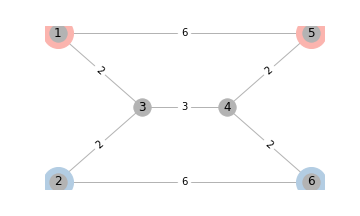
\includegraphics[width=8cm]{../resources/example_1_base.png}
  \caption{Representación de la red utilizada para el ejemplo de aplicación del problema. Los dos pares origen-destino se detallan con un color diferente. Cada arco tiene una etiqueta con el costo de usuario sobre la red de calles.}
  \label{fig:example1base}
\end{figure}

Podemos deducir de la Figura \ref{fig:example1base}, que el camino más corto para ambos pares origen-destino sobre la red de calles está compuesto por un solo arco de costo 6. El objetivo entonces es decidir dónde construir tecnología 1 tal que el costo de los caminos más cortos de uno o ambos pares origen-destino sea menor a 4 unidades (dada la función de transferencia de demanda), de manera que una cantidad $D$ o $2D$ de demanda total pueda ser transferida a la bicicleta. Nótese que los valores posibles de demanda transferida total en este caso solo pueden ser $0$, $D$ y $2D$. Si decidimos utilizar tecnología 1 en alguno de los arcos (1, 5) o (2, 6), digamos el primero, entonces nos aseguramos que la demanda del par origen-destino (1, 5) será transferida a la bicicleta, ya que el costo del camino más corto pasa a ser $3$. Con el presupuesto remanente de valor $5$, solamente podremos construir tecnología 1 en a lo sumo dos de los arcos (2, 3), (3, 4) y (4, 6). No es difícil ver que a lo sumo podremos mejorar el costo del camino más corto a $4.5$ para el par origen-destino (2, 6). La demanda transferida total en este caso es entonces de $D$.

La solución óptima consiste en construir tecnología 1 en todos los arcos del grafo menos los (1, 5) y (2, 6). Esto permite que ambos pares origen-destino tengan un nuevo recorrido como camino más corto, de costo $3.5$, lo que permite, según la función de transferencia de demanda, transferir $2D$ unidades de demanda. Esta solución se puede observar gráficamente en la Figura \ref{fig:example1solution}. El hecho de que los caminos más cortos circulen únicamente por arcos donde hay tecnología 1 es casual y pueden existir, en otras instancias, soluciones óptimas cuyos flujos circulen en parte por la red de calles.

\begin{figure}[h!]
  \centering
  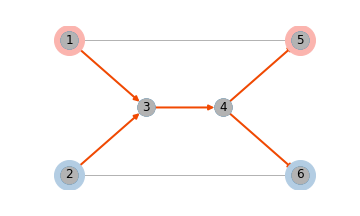
\includegraphics[width=8cm]{../resources/example_1_infras.png}
  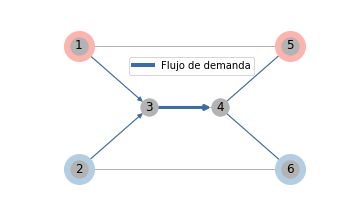
\includegraphics[width=8cm]{../resources/example_1_flows.png}
  \caption{Representación de la solución óptima en el grafo. Arriba se muestra en naranja en cuáles arcos se construye la tecnología 1. Abajo, en azul, los flujos sobre los caminos más cortos para ambos pares origen-destino. Nótese que el ancho del arco en este caso da una noción de la cantidad flujo.}
  \label{fig:example1solution}
\end{figure}

\FloatBarrier
\clearpage
\section{Formulación matemática de dos niveles}

Presentamos la formulación matemática. Sean los siguientes conjuntos, parámetros y variables:

\begin{description}
  \item[$I$]: Conjunto índice de tipos de tecnologías de ciclovías, numeradas desde $0$ en adelante. Se cumple que a mayor valor del índice mejor es la tecnología para el usuario, es decir tiene menor costo de usuario, y mayor el costo de construcción. El índice 0 corresponde a la calle y representa la no construcción de infraestructura de ciclovía.
  \item[$A_n^+$]: Conjunto de arcos que salen del nodo $n \in N$, $A_n^+ \subseteq A$.
  \item[$A_n^-$]: Conjunto de arcos que entran al nodo $n \in N$, $A_n^- \subseteq A$.
  \item[$C_{ai}$]: Parámetro que modela el costo de usuario de atravesar el arco $a \in A$ utilizando la tecnología $i \in I$, $C_{ai} > 0$.
  \item[$H_{ai}$]: Parámetro que modela el costo de construcción de la tecnología $i \in I$ sobre el arco $a \in A$, $H_{ai} \geq 0$.
  \item[$B$]: Parámetro que contiene el valor de presupuesto de construcción de infraestructura de ciclovía, expresado en las mismas unidades de los valores $H_{ai}$.
  \item[$\theta_{nk}$]: Parámetro que vale 1 si $n \in N$ es el origen del par origen-destino $k \in OD$, -1 si es el destino y 0 en otro caso.
  \item[$y_{ai}$]: Variable binaria de primer nivel que determina si la tecnología $i \in I$ está activa, es decir construida, en el arco $a \in A$. La representamos con el vector $y$ en la maximización de primer nivel.
  \item[$x'_{ak}$]: Variable de segundo nivel que determina si el arco $a \in A$ es parte del camino más corto para el par origen-destino $k \in OD$. La representamos con el vector $x'$ en la minimización de segundo nivel.
  \item[$x_{ak}$]: Variable de primer nivel que toma el valor de $x'_{ak}$ en la solución óptima del problema de segundo nivel. La representamos con el vector $x$ en la minimización de primer nivel.
  \item[$w_k$]: Variable de primer nivel que contiene el valor del camino más corto para el par origen-destino $k \in OD$ una vez que se impactan las decisiones dadas por $y_{ai}$. La representamos con el vector $w$ en la maximización de primer nivel.
  \item[$f_k$]: Función que determina la demanda que utiliza la bicicleta como modo de transporte en función del costo del camino más corto para el par origen-destino $k \in OD$.
\end{description}

Definimos la siguiente formulación de programación matemática:

\begin{align}
  \max_{w,x,y}   & \sum_{k \in OD} f_k(w_k)                                                         & \label{eq:objective1lvl} \\
  \text{s.t.}\;  & \sum_{a \in A} \sum_{k \in OD} \sum_{i \in I} C_{ai}y_{ai}x_{ak} = w_k           & \forall k \in OD \label{eq:shortestpath} \\
                 & \sum_{a \in A} \sum_{i \in I} H_{ai}y_{ai} \leq B                                & \label{eq:respectbudget} \\
                 & \sum_{i \in I} y_{ai} = 1                                                        & \forall a \in A \label{eq:alwaysoney} \\
                 & y_{ai} \in \{0,1\}                                                               & \forall a \in A, i \in I \nonumber \\
                 & x \in \argmin_{x'} \sum_{a \in A} \sum_{k \in OD} \sum_{i \in I} C_{ai}y_{ai}x'_{ak}  & \label{eq:subproblem} \\
                 & \qquad \text{s.t.} \sum_{a \in A_n^+} x'_{ak} - \sum_{a \in A_n^-} x'_{ak} = \theta_{nk}   & \forall n \in N, k \in OD \label{eq:flowbalance} \\
                 & \qquad \modelspace x'_{ak} \geq 0                                                          & \forall a \in A, k \in OD \nonumber
\end{align}

Donde:

\begin{description}
  \item[(\ref{eq:objective1lvl})]: Función objetivo de nivel superior, es la suma de los valores de demanda para cada par origen-destino que decidieron usar la bicicleta.
  \item[(\ref{eq:shortestpath})]: Restricción que determina el costo del camino más corto dado en el primer nivel, utilizada para facilitar la lectura del modelo.
  \item[(\ref{eq:respectbudget})]: Restricción de presupuesto sobre las tecnologías de ciclovías que pueden ser construidas.
  \item[(\ref{eq:alwaysoney})]: Restricción que requiere que una y solo una tecnología esté activa en cada arco.
  \item[(\ref{eq:subproblem}) y (\ref{eq:flowbalance})]: Función objetivo del segundo nivel y restricción de balance de flujo. Resuelven el problema del camino más corto para cada par origen-destino modelando el comportamiento de los usuarios.
\end{description}

\section*{Discusión sobre la formulación}

La formulación (\ref{eq:objective1lvl})-(\ref{eq:flowbalance}) denota un problema de programación binivel, o {\it BLPP} de sus siglas en inglés. Los problemas de primer y segundo nivel son llamados también líder y seguidor respectivamente. Estos nombres nos dan una idea de la jerarquía y de la naturaleza de esta formulación. Las variables relevantes del problema líder son las $y_{ak}$ que modelan los tipos de tecnologías construidos en cada arco y una vez que el líder selecciona un valor del vector $y = \left( y_{ak}: a \in A, k \in OD \right)$, estas variables se tornan constantes para el problema seguidor. La naturaleza secuencial de las decisiones implica que las variables de segundo nivel $x'_{ak}$ se pueden ver en función de $y$, es decir, $x' = x'(y)$, aunque en general no se usa esta notación \parencite{bardbook}. Omitimos en esta discusión las variables $w_k$ por ser un agregado de las variables $x_{ak}$ sobre $a \in A$.

Vale le pena mencionar que buscamos resolver en última instancia un problema de optimización lineal para poder acceder a métodos eficientes de resolución y aplicar el modelo a instancias de gran tamaño, como lo son las instancias reales. La formulación planteada en su estado actual no lo es por las ecuaciones (\ref{eq:shortestpath}) y (\ref{eq:subproblem}), y depende de la formulación explícita de las funciones $f_k$, $k \in OD$. Profundizaremos al respecto en el Capítulo \ref{sect:problemresolution}, página \pageref{sect:problemresolution}.

% \subsection{Costos y presupuesto}

Los parámetros más relevantes de la formulación son los que modelan los costos de usuario $C_{ai}$ y costos de construcción $H_{ai}$ para cada par de arcos y tipos de tecnologías de cilcovías. Para el problema de primer nivel, las decisiones sobre cuáles tecnologías construir están limitadas por el costo de construcción total, restricción (\ref{eq:respectbudget}). Las unidades de los costos de construcción por arco y tecnología $H_{ai}$ y presupuesto total $B$ son las mismas y pueden estar expresadas en cualquier unidad monetaria o valor que les de un carácter de bien económico. Por otro lado, los costos de usuario $C_{ai}$ son relevantes para el problema de segundo nivel, ya que es en función de estos que se realiza la optimización. El carácter de estos también es económico, porque dado un bien, por ejemplo trasladarse entre dos puntos de la red, a menor costo mejor; pero su interpretación está orientada a utilidad o beneficio que le brinda al usuario. Hay una relación entre los costos de construcción y los costos de usuario respecto a las tecnologías $I$ y es que a mayor costo de construcción (mejor tecnología) menor es el costo de usuario, considerado por unidad de distancia. Por ejemplo, construir una ciclovía pavimentada exclusiva para los ciclistas es más deseable para estos (y más costoso de construir) que una ciclovía que consiste en una sección de la calle reservada para el tránsito en bicicleta.

% \subsection{Modelado de tecnologías y caminos de los usuarios}

En la formulación del problema de primer nivel, la restricción (\ref{eq:alwaysoney}) pudo haber sido escrita de manera que a lo sumo una tecnología esté activa por arco, es decir, dejar la posibilidad de que no haya infraestructura en un arco. Esto se puede ver de diferentes maneras. Pensando en la realidad modelada, un ciclista podría circular prácticamente por cualquier calle sin problemas, entonces para que las instancias de la formulación (\ref{eq:objective1lvl})-(\ref{eq:flowbalance}) sean semánticamente correctas debería existir una tecnología $i_{base} \in I$ cuyo costo de construcción $H_{ai_{base}}$ sea 0 en todos de los arcos $a \in A$. Utilizamos el índice 0 para dicha tecnología, es decir $i_{base} = 0$. Desde un punto de vista formal, si no se requiere que en cada arco haya siempre una tecnología activa, se complejiza la formulación al representar de dos maneras los costos de usuario: por un lado, el costo de usuario de circular por la calle que es siempre permitido y por otro el costo de circular por una de las tecnologías especializadas si está activa. Por otro lado, si dejamos la posibilidad de que no haya tecnología activa en un arco, deberíamos agregar al problema de segundo nivel una restricción que evite flujos en arcos donde no hay infraestructura activa, es decir: $x_{ak} \leq \sum_{i \in I} y_{ai}, \forall a \in A, k \in OD$. Con esta restricción, el problema de segundo nivel puede no tener solución factible cuando las tecnologías seleccionadas por el primer nivel no induzcan un subgrafo que conecta todos los pares origen-destino, cosa que no es deseable desde el punto de vista de la validez del modelo binivel, ver demostraciones en el Apéndice \ref{sect:apendixbilevelvalidation}, página \pageref{sect:apendixbilevelvalidation}.

Asumiremos de aquí en adelante que las instancias del problema están bien definidas, esto significa que:

\begin{enumerate}
  \item {$G$ es conexo}
  \item {$\forall k \in OD$ existe un camino $S_k \in G$ con costo de construcción cero, es decir $\sum_{a \in S_k} H_{ai_0} = 0$}, donde $i_0$ es el tipo de tecnología de inversión nula.
\end{enumerate}

% \subsection{Modelado de la atracción de demanda}

Son de nuestro particular interés para la formulación los parámetros que representan la demanda y funciones de transferencia de demanda entre modos. Incurrimos en una simplificación que reduce varios modos de transporte (por ejemplo transporte público, taxi o privado) a uno, y consideramos la transferencia desde este modo agregado a la bicicleta. Por lo tanto, las funciones de transferencia de demanda son funciones de $\mathbb{R}^+$ en $\mathbb{R}^+$, cuyos valores del dominio están expresados en unidad del costo de usuario y sus valores del codominio en unidad de demanda que se transfiere de un modo a otro.

El modelo busca determinar la mayor transferencia de demanda entre dos modos de transporte. Para esto, consideramos que sobre la tecnología base la demanda transferida es cero, es decir, que el costo del camino más corto utilizando la bicicleta únicamente sobre la tecnología base no induce transferencia de demanda. Suponemos que partimos de un conjunto de demanda insatisfecha por la tecnología de ciclovías base, pero potencial, si las condiciones mejoran.

En el caso más general, la decisión de utilizar la bicicleta es multifactorial y depende principalmente de tres tipos de factores \parencite{ortuz2011}:

% Modeling Transport, Ortuzar 2011. Pag. 208
\begin{enumerate}
  \item{
      Características del viajante
        \begin{itemize}
          \item{Edad}
          \item{Nivel socio-económico}
          \item{Otros factores como utilización de auto para el trabajo, llevar niños a la escuela, etc.}
        \end{itemize}
  }
  \item{
      Características del viaje
        \begin{itemize}
          \item{Propósito}
          \item{Momento del día}
        \end{itemize}
  }
\item{\label{bicycleusagefactors}
      Características cuantitativas y cualitativas de las facilidades de transporte
      \begin{itemize}
          \item{Disponibilidad de transporte público}
          \item{Infraestructuras de ciclovías}
          \item{Costo del transporte público y combustibles}
          \item{Comodidad y conveniencia}
          \item{Seguridad y protección}
      \end{itemize}
  }
\end{enumerate}

En este trabajo nos concentramos en el punto \ref{bicycleusagefactors}, exclusivamente en los factores que pueden ser favorecidos por la presencia de ciclovías: infraestructura de ciclovías, comodidad y conveniencia, seguridad y protección. Cada tipo de tecnología de ciclovías puede afectar estos factores de distinta manera, pero siempre los modelamos como un único valor para cada arco mediante el parámetro $C_{ai}$. Sobre los otros factores, asumimos que solo consideramos el universo de demanda que es transferible a la bicicleta. Esto nos ahorra considerar aspectos como si el viaje se hace de noche o si el trabajo requiere un vehículo automotor.

El mecanismo de agregar diferentes factores en un único valor es el concepto de utilidad que se utiliza en los modelos probabilísticos de \textcite{ortuz2011, Pacheco2021}. A diferencia de dichos trabajos, en los que se buscan mayores niveles de utilidad, en el nuestro, al modelarlo como un costo, tenemos que menores valores son más deseables.

El modelado de la red de calles y los distintos tipos ciclovías lo realizamos de manera que sobre la red original puedan implantarse infraestructuras de ciclovías que modifican el costo de usuario de atravesar los arcos de la red. Luego configuramos el costo de usuario en cada arco dependiendo de la tecnología activa del arco. El mismo enfoque se utilizó en \parencite{Lin2013, Zhu2019}. Por otro lado, en \parencite{baya2021} el modelado de diferentes tecnologías de ciclovías se implementó como un grafo multicapas donde cada capa replica la red original. La primera capa es la red de calles, la siguiente capa corresponde a la tecnología de tipo 1 y así sucesivamente. Además, cada nodo está conectado con sus nodos réplica en las capas que corresponden a otras tecnologías. Mediante variables de activación permiten que solo una tecnología esté activa en cada arco de lo que representa la red original. Este diseño permite identificar los flujos que cambian de tipo de ciclovía durante un trayecto con el objetivo de penalizar dicho cambio. Notar que este enfoque también es aplicable a nuestro problema. La diferencia entre nuestro modelado y el de \textcite{baya2021} es que el primero modela los diferentes tipos de tecnología a nivel de formulación y el segundo a nivel de los datos.

  % \chapter{Metodología}

El objetivo de este capítulo es justificar el diseño metodológico elegido. La finalidad de una metodología bien descrita es explicitar los pasos mediante los cuales se obtienen los resultados, y por tanto el cumplimiento (o no) de los objetivos establecidos, de manera tal que pueda ser replicado por otro investigador. Si corresponde, también se evaluarán problemas metodológicos y se realizarán consideraciones éticas.
En algunas disciplinas este capítulo se denomina Materiales y métodos. 
En caso de que la investigación sea de carácter experimental, se debe especificar la siguiente información:


\begin{itemize}
\item	el tipo de investigación realizada (experimental, descriptiva, estudio de caso, encuesta de opinión, etc.)
\item	el modo de recolección de datos (análisis documental, observación participante o no, entrevista o cuestionario, etc.)
\item	población o sujetos experimentales.
\item	protocolo de investigación, si corresponde  
\end{itemize}

En algunas disciplinas formales no es pertinente la inclusión de un capítulo que recoja una cierta metodología de trabajo. En tales casos, se espera que el tesista haga mención de cuestiones carácter metodológico en la Introducción.

El procesamiento del trabajo metodológico que no es imprescindible para la comprensión del texto puede incluirse en apéndices o anexos (Anexo \ref{Ane1}).



 % Se carga el capítulo 03
  % \chapter{Presentación de los datos, Análisis, Discusión}

En algunas disciplinas, el capítulo Presentación de datos va acompañado del análisis o de la discusión de la información (\textit{Presentación y análisis de los datos}; \textit{Resultados y discusión}), en tanto que en otras, \textit{Presentación}, \textit{Análisis} y \textit{Discusión} son capítulos separados.
El objetivo de esta(s) parte(s) de la tesis es presentar los datos recabados y el análisis realizado a la luz de la bibliografía ya revisada. Se puede incluir la interpretación de los resultados (\textit{Discusión}) a partir del análisis de los datos, o también relacionarlos con estudios relevantes que se entienden pertinentes, aun si estos no se han consignado en los \textit{Fundamentos teóricos}, ya que se entiende que al analizar los datos pueden aparecer algunos que no se enmarcan teóricamente o que no se explican en el encuadre teórico o en estudios ya existentes.

Ahora a modo de ejemplo mencionamos el símbolo de los números reales utilizando el comando \verb|\gls{}| \gls{Real} y el comando \verb|\glssymbol{}| \glssymbol{Real}. Otro ejemplo es mencionar el tensor simétrico de tensiones \gls{sigma}, o un valor escalar  \gls{alph} o un conjunto vacío \gls{emptyset}.

\newpage 


\section{Título de sección}

Ejemplo de tabla

\begin{table}[h!]
\centering
\caption{Leyenda de tabla.}
\label{tab:comp}
\begin{tabular}{|c|c|c|}
  \hline
  $t$ (seg) & $x$(t) & $y$(t)\\
  \hline
  1 & 0.0000 & 0.0001\\
  2 & 0.5000 & 0.2498\\
  3 & 1.0000 & 1.0000\\
  4 & 1.5000 & 2.2403\\
  5 & 2.0000 & 4.0010\\
  6 & 2.5000 & 6.2459\\
  \hline
\end{tabular}
\end{table}

Ejemplo de figura.

\begin{figure}[h!]
\label{fig:comp}
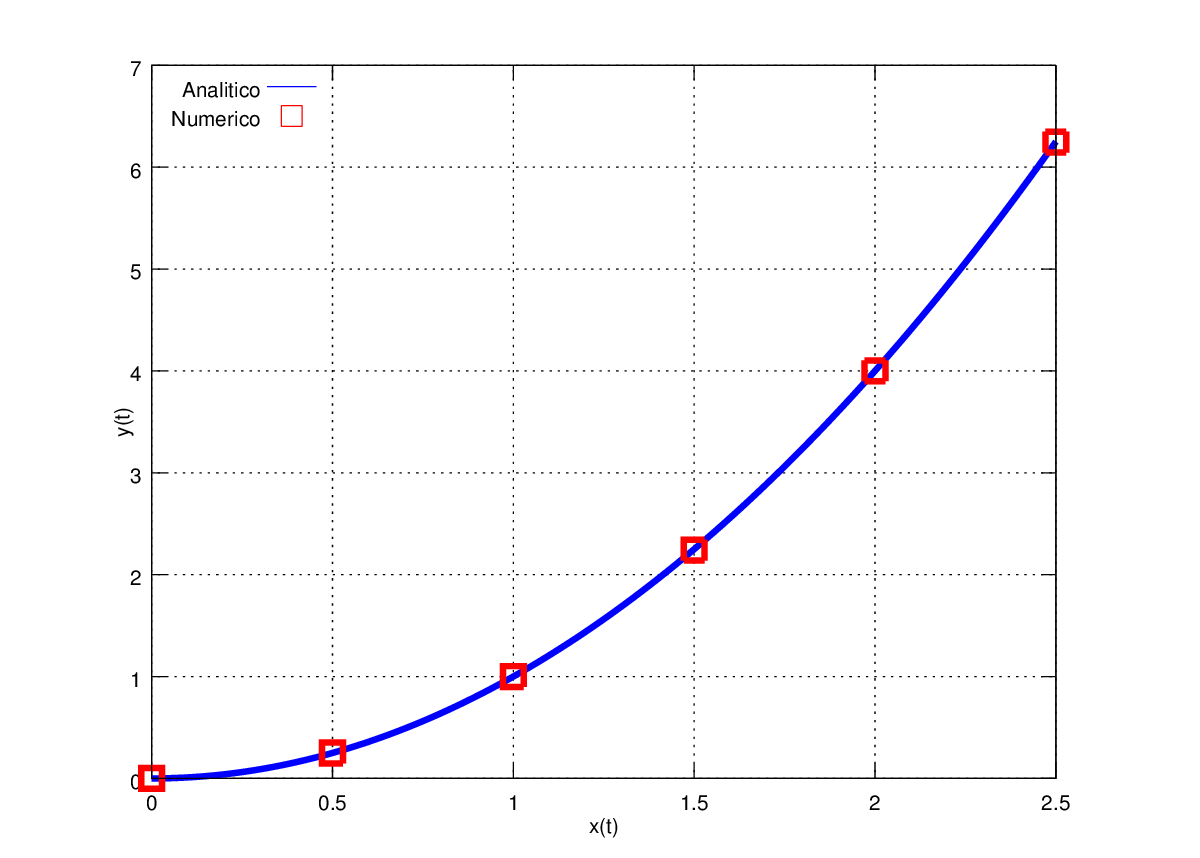
\includegraphics[width=.8\textwidth]{imagenes/chap4/x_vs_y}
\caption{Leyenda de figura.}
\end{figure}
Ejemplo de ecuación:
\begin{equation}
y(x)=x^2
\end{equation}
 % Se carga el capítulo 04
  % \chapter{Consideraciones finales}

En este capítulo se sintetizan las posturas expuestas en el capítulo anterior. Se retoma la pregunta de investigación y se expresa si los resultados apoyan o no la hipótesis planteada. 

Además, se pueden hacer contribuciones teóricas o metodológicas a la disciplina y recomendaciones para trabajos futuros o para profundizar en el campo, plantear nuevas interrogantes o proponer explicaciones \textit{post hoc}. En algunos trabajos este capítulo se subdivide en otras secciones que presentan algunos de los contenidos mencionados. 
En algunas tradiciones académicas este capítulo recibe distintas denominaciones: \textit{Conclusiones}, \textit{Conclusiones y trabajos a futuro}, \textit{Consideraciones finales y recomendaciones}. 

 % Se carga el capítulo 05
 % Seguir copiando la linea de arriba para agregar más capítulos.

  \backmatter % Comando que generalos apéndices, anexos y bibliografía. NO COMENTAR

  \bibliography{bibliografia/tesis,bibliografia/ambicycle} % Agregar la cantidad de archivos .bib que se tengan para la bibliografía.
  \bibend % No comentar
  % 
  \glosario % Glosario, NO comentar
  %
  \apenarabicnumbering
  \apenmatter % Apéndices, NO comentar
  \chapter{Datos procesados}


  \chapter{Imágenes remasterizadas}\label{Ape2}

  \chapter{Entrevistas desgrabadas}\label{Ape3}


  % Seguir copiando la linea de arriba para agregar más apéndices.

  \anexarabicnumbering
  \anexmatter % Anexos, NO comentar
  %  \chapter{Material legislativo}\label{Ane1}

XXXXX
  % Seguir copiando la linea de arriba para agregar más anexos.
  %
\end{document}

% ===== FIN DEL DOCUMENTO =====
